\subsection{Detección de marcadores}
El bloque de detección de marcadores, se puede dividir en dos partes: la \textit{segmentación} y el \textit{filtrado de objetos}.
%
El algoritmo realiza la detección siguiendo el siguiente proceso:
%
\begin{enumerate}
  \item Obtención de cada cuadro de la entrada de video.
  \item Se toma un cuadro y se segmenta utilizando umbralización de Otsu.
  \item A partir de la imagen segmentada, se identifican los marcadores.
  \item Se escribe la posición de los marcadores detectados en un archivo XML.
  %\item Se escribe la posición de los marcadores detectados para este cuadro en un archivo con formato XML.
  \item Se toma el siguiente cuadro y se repite el proceso a partir del paso 2.
\end{enumerate}
\vspace{-0.4cm} 
\subsubsection{Descripción de las etapas de detección.}
El bloque de \textit{segmentación} utilizó umbralización generando umbrales con el método de Otsu\cite{otsu} de tres clases.\\
%
La etapa de \textit{filtrado} no es más que una clasificación de los objetos segmentados. Dado que los objetos a detectar tienen formas relativamente sencillas (círculos blancos sobre fondo oscuro) y las condiciones de laboratorio son controladas al realizar la captura, esta etapa no requirió implementar algoritmos muy complejos. En particular, se implementó un detector de objetos circulares en base a momentos geométricos\cite{imageMoments} y un filtro según el área de los mismos.
\vspace{-0.3cm} 
\subsubsection{Resultados.}
En la etapa de segmentación se observó que el resultado obtenido depende fuertemente de las condiciones de captura y del umbral calculado. Si las condiciones de captura se apartan de las definidas en la sección \ref{section_base_de_datos}, los resultados pueden no ser satisfactorios. Sin embargo, si las capturas se hacen dentro de las condiciones establecidas, los resultados obtenidos son aceptables, como se observa en la Figura \ref{ejemploabelumbr2}.

\begin{figure}[ht!]
      \centering
        \subfloat[]{{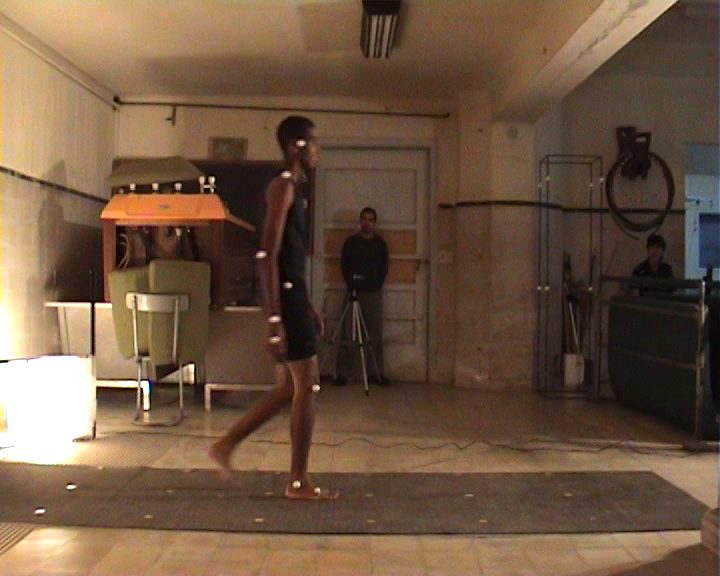
\includegraphics[trim = 5mm 0mm 2mm 0mm, clip, scale=0.21]{imagenes/abel_original_video.png}\label{abelvideo}}}\hspace{6 mm}
        \subfloat[]{{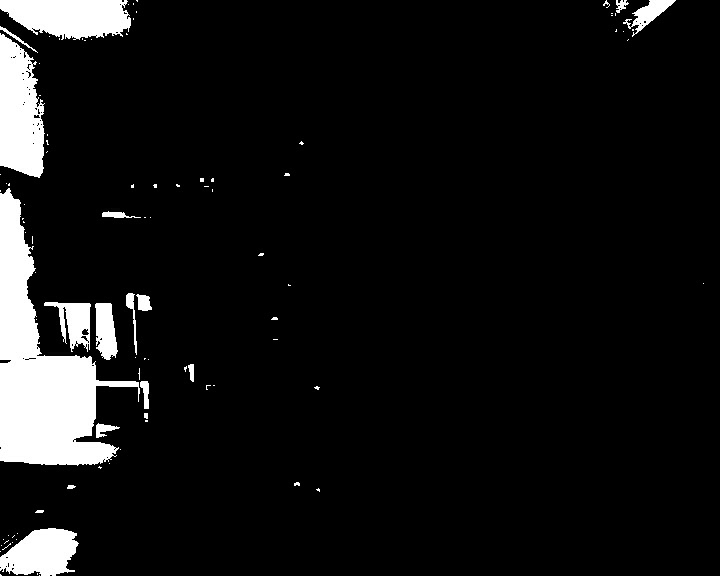
\includegraphics[scale=0.21]{imagenes/abel_original_filtro.png}\label{abelfiltro}}}\hspace{2 mm}
        \subfloat[]{{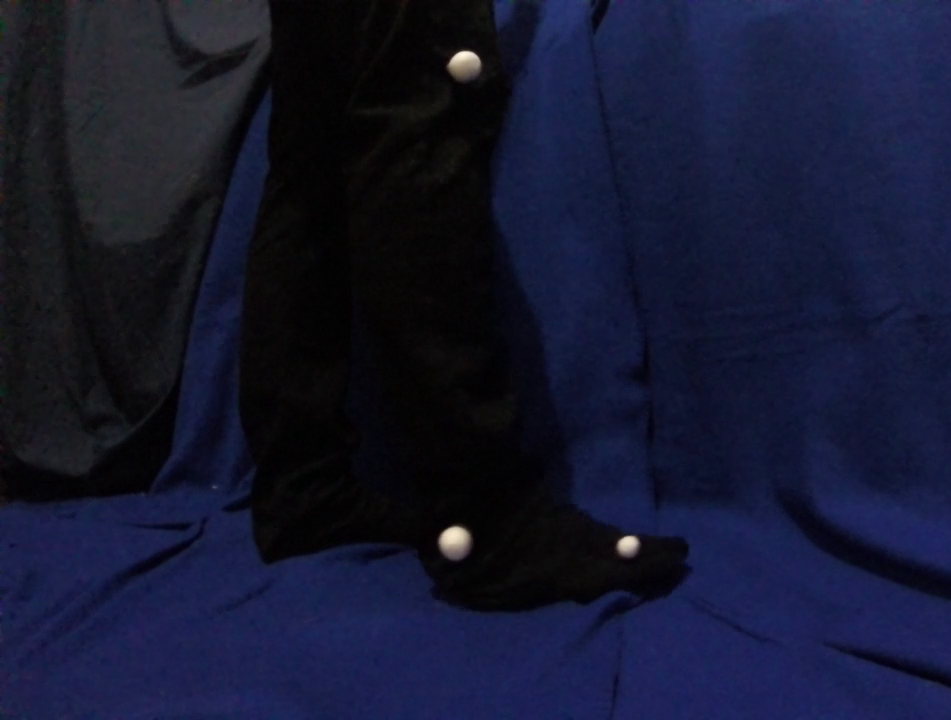
\includegraphics[trim = 5mm 0mm 5mm 0mm, clip, scale=0.16]{imagenes/orig.png}\label{abelvideo2}}}\hspace{4.9 mm}
       % {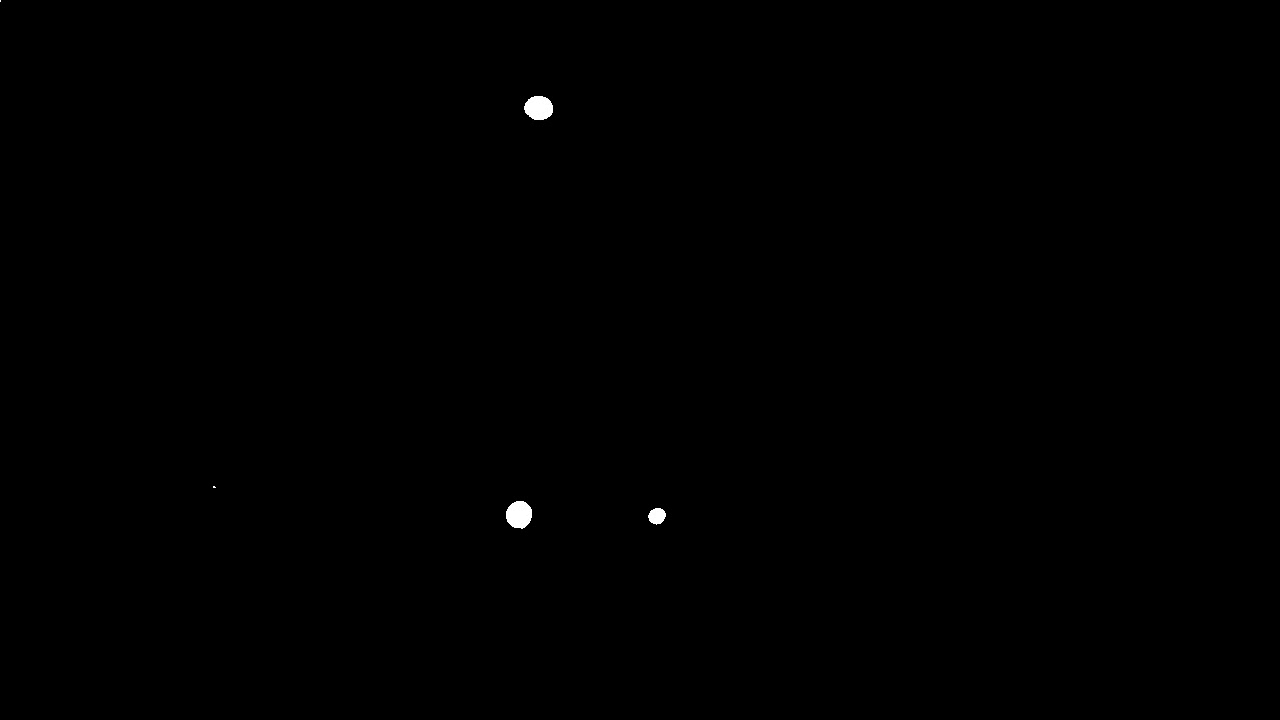
\includegraphics[scale=0.07]{imagenes/filtr.png}\label{abelfiltro2}}\hspace{1 mm}
        \subfloat[]{{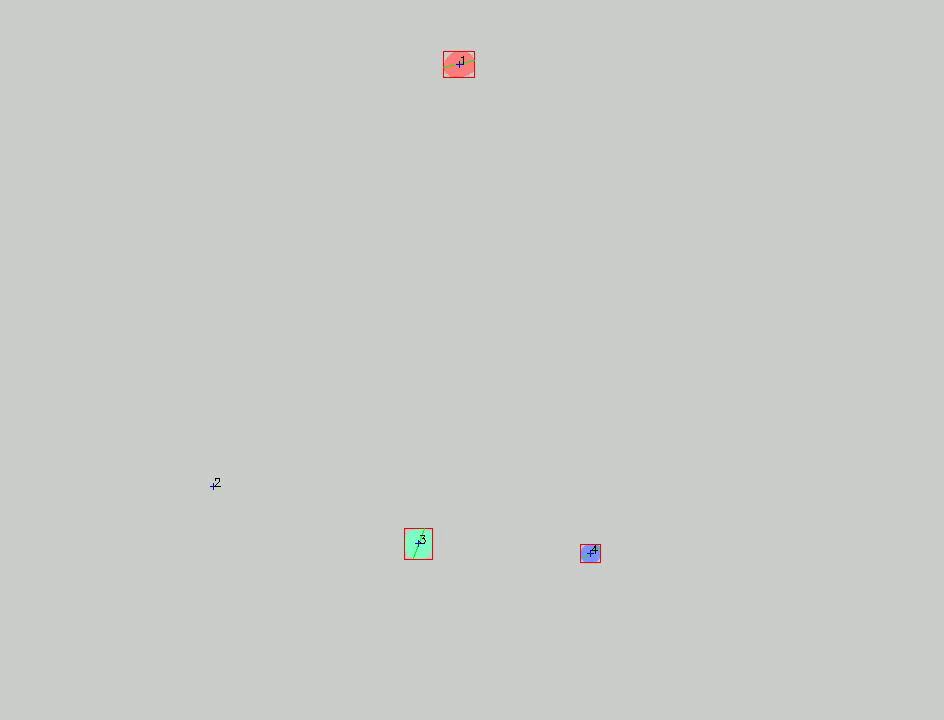
\includegraphics[trim = 5mm 0mm 0mm 07mm, clip, scale=0.164]{imagenes/detect.png}
        \label{abeldetect}}}
      \caption{%Entradas y salidas de cada etapa del bloque de deteción.
       %\textbf{(\ref{abelvideo})} 
       {(a)} Imagen original de una secuencia fuera de las hipótesis de captura. 
       (b) Resultado de la segmentación fuera de las hipótesis de captura.
       % \textbf{(\ref{abelvideo2})} 
       (c) Captura original de una secuencia real bajo las hipótesis de captura.
       % \textbf{(\ref{abelfiltro2})} Imagen filtrada con el umbral de Otsu. \textbf{(\ref{abeldetect})}
       (d) Marcadores detectados.}  
      \label{ejemploabelumbr2}
\end{figure}
